\chapter{Background}
\label{chap:background}

The readers benefit from an understanding regarding the state-of-the-art and 
the current challenges presented in the field of parallel computing and deep 
learning in order to grasp the works carried out from this thesis.
This chapter prepares the reader with the acquaintances of the various forms of 
modern parallel systems and the task-based programming paradigm for such systems. 
This chapter subsequently presents an introduction to the two application domains
this work deals with, namely, parallel numerical algorithms and DNNs.

\section{Modern Parallel Systems}
The Exascale supercomputers are expected to come into operation near 
2020. In order to reach that, major improvements need to be achieved including 
the energy and power, memory and storage, concurrency and locality and 
resiliency~\cite{doe}. Nevertheless, the mainstream trend stays with the massive 
parallelism with accelerators approach. This section provides a background on 
both types of systems and an introduction to some major parallel programming 
paradigms.

With the roll-out of 7 and 5 nm node, the VLSI (very large scale integration) 
manufacturing technology is rapidly approaching its end due to its physical 
limitation. Furthermore, the power and energy consumption, as a consequence the 
heat dissipation, on a modern VLSI chip has become a major limiting factor in 
processor design. All the above impede the efforts to push a single-core 
processor to go faster. In response, industry turns its attention into 
designing multi-core multiprocessor systems which exploit parallelism at the 
application level. Figure~\ref{fig:multicore} illustrates a typical multi-core 
multiprocessor system~\cite{ibm_multicore}. Each of the processor (processor 0 
and 1) packs two separate cores with their own L1 and L2 cache. The two 
processors are connected via a system bus which also connects to the RAM. All 
the cores thus are able to access to the entire memory region. Nonetheless, 
since all the access to the memory and communication among processors are 
conducted on the system bus, the system is limited in its scale in that the 
inevitable contention on the bus system while the number of processors grows 
eventually renders a large-scale system unresponsive.
\begin{figure}[H]
    \centerline{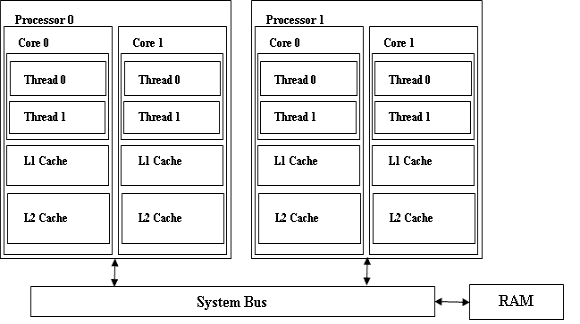
\includegraphics[scale=0.50]{background/figs/multicore_mp_system.png}}
    \caption{A typical chip multithreaded, multi-core, multiprocessor system}
    \label{fig:multicore}
\end{figure}

With the evergrowing demand of computation power, a large amount of such 
processors are grouped close together into a computer cluster with high speed 
interconnection system to further scale the system. All the cores belonging to 
the same node in the cluster shares the resources (memory system, last-level 
cache etc.) whereas cross-node resources are private to their respective nodes. 
This essentially segragates the memory system into various regions not directly 
accessable to all the cores. Accessing remote contents is possible by sending 
them as message to the requesting node which implies that accessing to different 
memory regions incurs distinct latency.  This offloads the task of ensuring the 
performance of the program to the programmer because careless handling of the 
physical location and topology of the nodes can easily saturate the 
interconnection system and cause processors to have imbalanced accessing time to 
the same data.

\subsection{Parallel Programming Models}
\subsubsection{Shared-Memory Programming Model}
OpenMP~\cite{openmp, OpenMP4.0} is a standard programming model on a 
shared-memory system. It is an application programming interface (API) that 
supports shared memory multiprocessing programming in C, C++, and FORTRAN.
\begin{figure}[H]
    \centerline{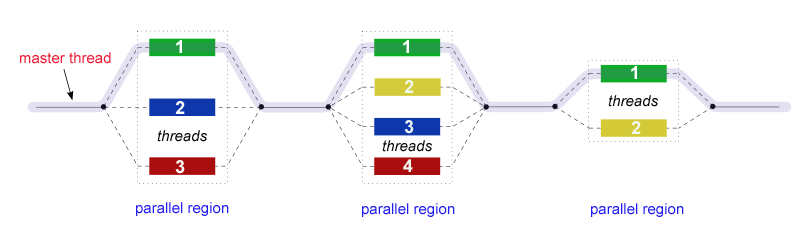
\includegraphics[scale=0.50]{background/figs/fork_join.png}}
    \caption{OpenMP uses a fork-join model}
    \label{fig:fork-join}
\end{figure}
OpenMP uses a fork-join model for its parallel executions as seen in 
Figure~\ref{fig:fork-join}.
All OpenMP programs begin as a single process: the master thread. The master 
thread executes sequentially until the first parallel region construct is 
encountered. The master thread then creates a team of parallel threads.
The statements in the program that are enclosed by the parallel region construct 
are then executed in parallel among the various team threads. When the team 
threads complete the statements in the parallel region construct, they 
synchronize and terminate, leaving only the master thread~\cite{llnl_openmp}.

\subsubsection{Task-based Parallel Programming Model}
This paradigm introduced 

\subsubsection{Distributed-Memory Programming Model}

\section{Numerical Solvers For Systems of Linear Equations}
\subsection{Direct Methods}
\subsection{Iterative Methods}

\section{Deep Neural Networks and Their Parallelization}
\subsection{Supervised Deep Learning}
\subsection{Data Parallelism}
\subsection{Model Parallelism}
